\documentclass[../../main/main.tex]{subfiles}
\graphicspath{{./figures/}}

\dominitoc
\faketableofcontents

\makeatletter
\renewcommand{\@chapapp}{M\'ecanique -- chapitre}
\makeatother

% \toggletrue{student}
% \HideSolutionstrue
% \toggletrue{corrige}
% \renewcommand{\mycol}{black}
% \renewcommand{\mycol}{gray}

\begin{document}
\setcounter{chapter}{5}

\settype{prof}
\settype{stud}
\settype{book}

\chapter{Moment cin\'etique pour un point mat\'eriel}

\vspace*{\fill}

\begin{prgm}
	\small
	\begin{tcb}*(ror)"know"{Savoirs}
		\begin{itemize}
			\item Moment cinétique d'un point matériel par rapport à un point et par
			      rapport à un axe orienté.
			\item Moment cinétique d'un système discret de points par rapport à un axe
			      orienté.
			\item Moment d'une force par rapport à un point ou un axe orienté.
			\item Théorème du moment cinétique en un point fixe dans un référentiel
			      galiléen.
			\item Conservation du moment cinétique.
		\end{itemize}
	\end{tcb}
	\begin{tcb}*(ror)"how"{Savoir-faire}
		\begin{itemize}
			\item Relier la direction et le sens du vecteur moment cinétique aux
			      caractéristiques du mouvement.
			\item Utiliser le caractère algébrique du moment cinétique scalaire.
			\item Calculer le moment d'une force par rapport à un axe orienté en
			      utilisant le bras de levier.
			\item Identifier les cas de conservation du moment cinétique.
		\end{itemize}
	\end{tcb}
\end{prgm}

% \vspace*{\fill}

% \newpage

\vspace*{\fill}
\minitoc
\vspace*{\fill}

\newpage

\vspace*{\fill}
\begin{boxes}
	\begin{tcb}(defi)<lftt>{Liste des définitions}
		\tcblistof[\paragraph*]{defi}{\hspace*{6pt}}
	\end{tcb}
	% \begin{tcb}(rapp)<lftt>{Liste des rappels}
	% 	\tcblistof[\paragraph*]{rapp}{\hspace*{6pt}}
	% \end{tcb}
	\begin{tcb}(prop)<lftt>{Liste des propriétés}
		\tcblistof[\paragraph*]{prop}{\hspace*{6pt}}
		\tcblistof[\paragraph*]{theo}{\hspace*{6pt}}
	\end{tcb}
	% \begin{tcb}(coro)<lftt>{Liste des corollaires}
	% 	\tcblistof[\paragraph*]{coro}{\hspace*{6pt}}
	% \end{tcb}
	\begin{tcb}(demo)<lftt>{Liste des démonstrations}
		\tcblistof[\paragraph*]{demo}{\hspace*{6pt}}
	\end{tcb}
	\begin{tcb}(inte)<lftt>{Liste des interprétations}
		\tcblistof[\paragraph*]{inte}{\hspace*{6pt}}
	\end{tcb}
	% \begin{tcb}(tool)<lftt>{Liste des outils}
	% 	\tcblistof[\paragraph*]{tool}{\hspace*{6pt}}
	% \end{tcb}
	% \begin{tcb}(nota)<lftt>{Liste des notations}
	% 	\tcblistof[\paragraph*]{nota}{\hspace*{6pt}}
	% \end{tcb}
	\begin{tcb}(appl)<lftt>{Liste des applications}
		\tcblistof[\paragraph*]{appl}{\hspace*{6pt}}
	\end{tcb}
	\begin{tcb}(rema)<lftt>{Liste des remarques}
		\tcblistof[\paragraph*]{rema}{\hspace*{6pt}}
	\end{tcb}
	% \begin{tcb}(exem)<lftt>{Liste des exemples}
	% 	\tcblistof[\paragraph*]{exem}{\hspace*{6pt}}
	% \end{tcb}
	\begin{tcb}(ror)<lftt>{Liste des points importants}
		\tcblistof[\paragraph*]{ror}{\hspace*{6pt}}
	\end{tcb}
	% \begin{tcb}(impo)<lftt>{Liste des erreurs communes}
	% 	\tcblistof[\paragraph*]{impo}{\hspace*{6pt}}
	% \end{tcb}
\end{boxes}
\vspace*{\fill}
\newpage

Jusqu'à présent, nous avons vu deux méthodes de résolution en mécanique~:
\begin{itemize}
	\item Le PFD au chapitre 2, pour avoir toute l'information sur un
	      mouvement~;
	\item Les théorèmes énergétiques (TEC et TEM, TPC et TPM) au chapitre 4,
	      pour les informations à un instant donné.
\end{itemize}
Il existe une autre méthode de résolution dans le cas spécifiques des
\textbf{mouvements de rotation}~: le théorème du moment cinétique. Dans ce
chapitre, \textbf{nous ne nous intéressons qu'à des points matériels M} de masse
$m$~: le traitement des solides viendra un peu plus tard.

\section{Moment d'une force}
\subsection{Par rapport à un point}
\begin{itemize}
	\item Lorsqu'une masse $m$ est placée à distance d'un point «~pivot~», cette
	      masse génère une rotation.
	\item On peut compenser cette rotation en mettant une même masse à la même
	      distance de l'autre côté.
	\item On peut compenser une masse plus grande en mettant une masse plus
	      faible plus loin du pivot.
	\item Ainsi l'effet est proportionnel à la distance au pivot.
\end{itemize}

\begin{isd}
	\begin{center}
		\sswitch{
			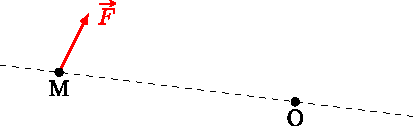
\includegraphics[scale=1, draft=true]{intro_perp}
		}{
			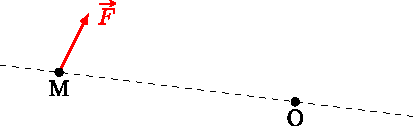
\includegraphics[scale=1]{intro_perp}
		}
		\captionof{figure}{$\protect\Ff$ tend à faire tourner M autour de O dans le
			sens horaire.}
	\end{center}
	\tcblower
	\begin{center}
		\sswitch{
			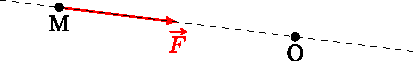
\includegraphics[scale=1, draft=true]{intro_parr}
		}{
			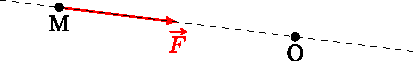
\includegraphics[scale=1]{intro_parr}
		}
		\captionof{figure}{$\protect\Ff$ ne cause aucune rotation.}
	\end{center}
\end{isd}

Pour traduire cette capacité d'une force à créer un mouvement de rotation autour
de O, on introduit une grandeur appelée \textbf{moment d'une force}.

\begin{tcb*}[sidebyside, righthand ratio=.2](defi){Moment d'une force}
	Le moment d'une force $\Ff$ au point M par rapport à un point O est le
	\textbf{vecteur}~:
	\psw{
		\[\boxed{\Mcf_{\Or}(\Ff) = \OM\wedge\Ff}\]
	}
	\tcblower
	\tcbsubtitle{\fatbox{\textbf{Unité}}}
	\[
		\psw{
			\si{J} = \si{N.m}
		}
	\]
\end{tcb*}

\begin{tcb*}(inte){Moment par rapport à un point~: géométriquement}
	La \textbf{direction} de $\Mcf_{\Or}(\Ff)$ indique la manière dont la force
	$\Ff$ a tendance à faire tourner M autour de O, et est donné par la
	\textbf{règle de la main droite}.
	\begin{center}
		\begin{tabularx}{\linewidth}{Y|Y|Y}
			\sswitch{
				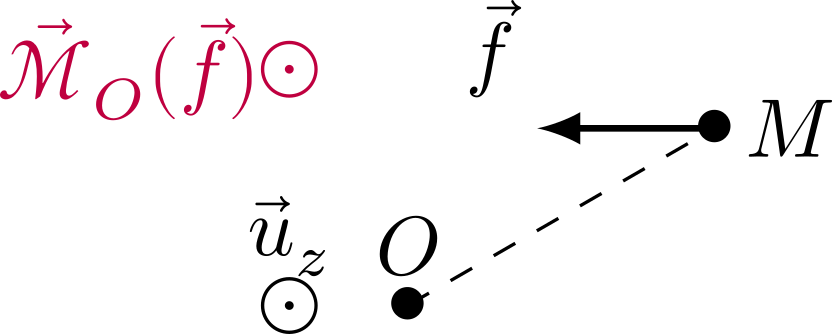
\includegraphics[scale=1, draft=true]{moment_force-a}
			}{
				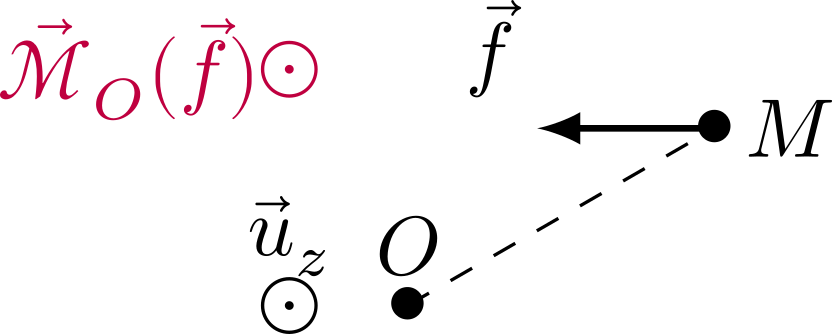
\includegraphics[scale=1]{moment_force-a}
			}
			 &
			\sswitch{
				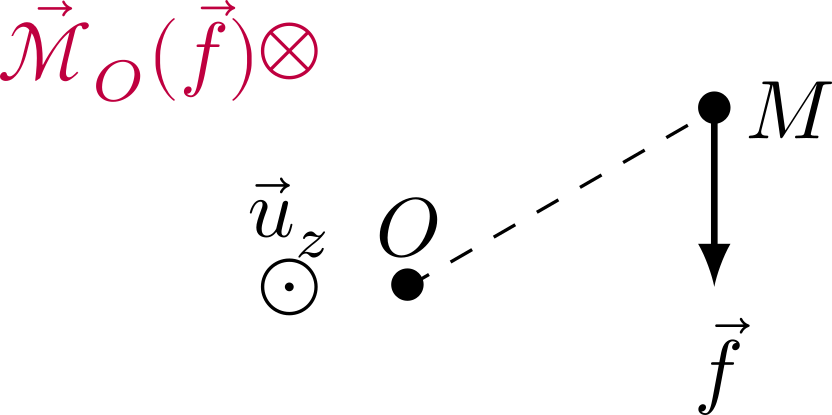
\includegraphics[scale=1, draft=true]{moment_force-b}
			}{
				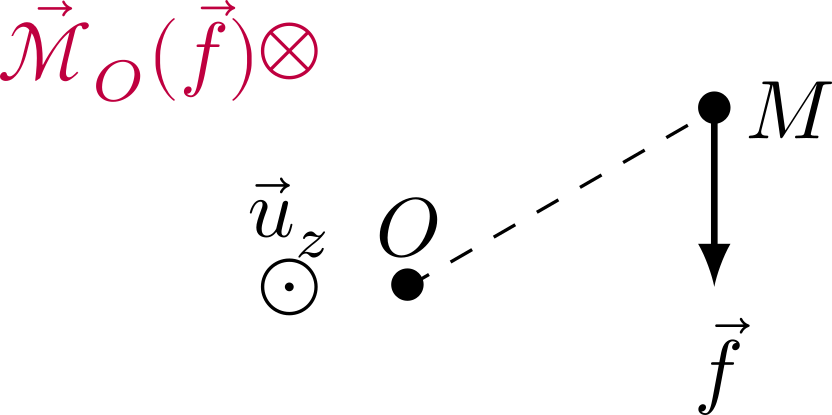
\includegraphics[scale=1]{moment_force-b}
			}
			 &
			\sswitch{
				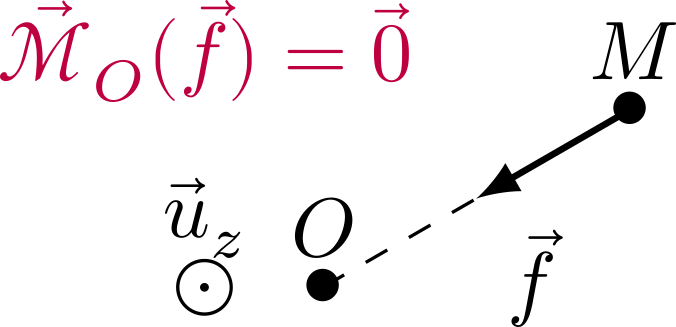
\includegraphics[scale=1, draft=true]{moment_force-c}
			}{
				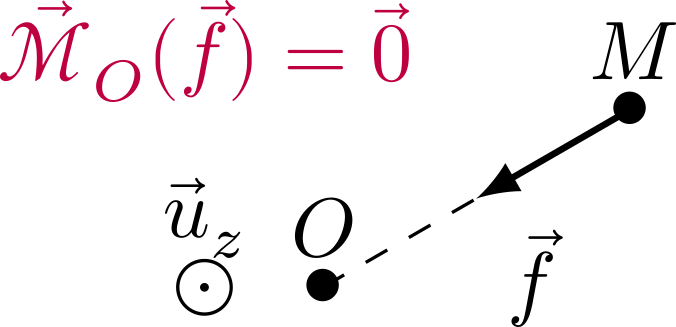
\includegraphics[scale=1]{moment_force-c}
			}
			\\[1em]
			\psw{
				Si $\Mcf_{\Or}(\Ff)$ est dirigé selon $+\uz$, $\Ff$ fait tourner M dans
				le sens \textbf{direct}.
			}
			 &
			\psw{
				Si $\Mcf_{\Or}(\Ff)$ est dirigé selon $-\uz$, $\Ff$ fait tourner M dans
				le sens \textbf{horaire}.
			}
			 &
			\psw{
				Si $\Mcf_{\Or}(\Ff) = \of$, $\Ff$ ne fait pas tourner M autour du point
				O.
			}
		\end{tabularx}
	\end{center}
\end{tcb*}

\begin{tcb*}(appl)<lftt>'l'{Moment du poids}
	\begin{minipage}[c]{0.70\linewidth}
		Un véhicule assimilé à un point matériel M de masse $m$ se déplace de
		haut en bas d'une colline~; la trajectoire est assimilée à un quart de
		cercle vertical de centre O et de rayon $R$. On note $\th$ l'angle que
		fait OM avec la verticale. Calculer le moment du poids par rapport à O.
	\end{minipage}
	\hfill
	\begin{minipage}{0.25\linewidth}
		\begin{center}
			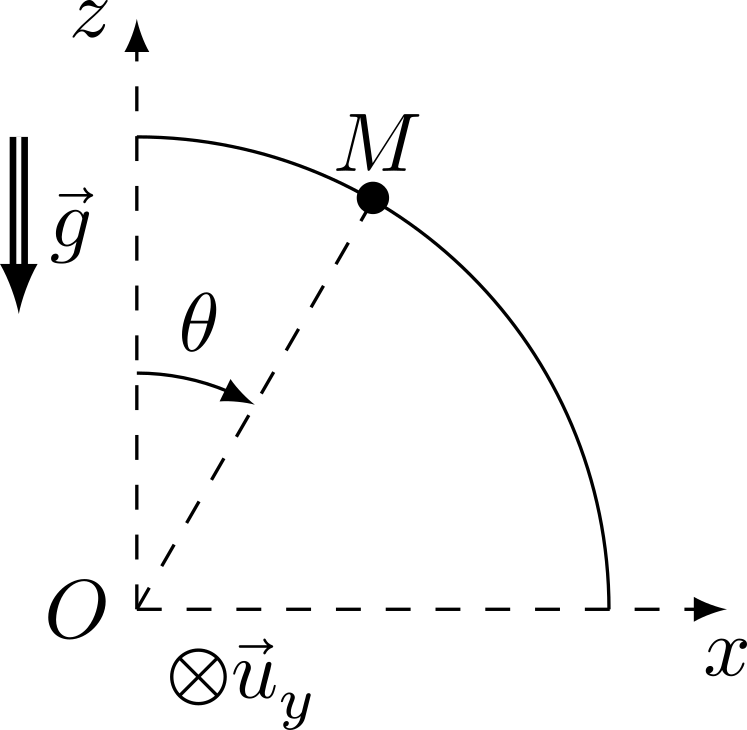
\includegraphics[scale=1]{moment_force-ex}
		\end{center}
	\end{minipage}
	\tcblower
	\psw{
		Pour calculer le moment d'une force, on décompose ladite force et le vecteur
		$\OM$ \textbf{dans la même base}. Ici, le poids s'exprime en coordonnées
		cartésiennes~: on projette donc la position $\OM$ dans le repère cartésien.
		On obtient ainsi~:
		\begin{gather*}
			\left\{
			\begin{aligned}
				\Pf & = -mg\uz                            \\
				\OM & = R\ur = R(\cos\th\uz + \sin\th\ux)
			\end{aligned}
			\right.
		\end{gather*}
		On peut donc calculer le moment du poids~:
		\begin{align*}
			\Mcf_{\Or}(\Pf) & = \OM\wedge\Pf                                       \\
			                & = -mgR(\cos\th\uz + \sin\th\ux)\wedge\uz             \\
			                & = -mgR\cos\th\underbracket[1pt]{\uz\wedge\uz}_{=\of}
			-mgR\sin\th\underbracket[1pt]{\ux\wedge\uz}_{=-\uy}                    \\
			\Lra
			\Aboxed{
			\Mcf_{\Or}(\Pf) & = +mgR\sin\th\uy
			}
		\end{align*}
		On vérifie \textbf{systématiquement} que la direction du moment donne bien
		le sens de rotation attendu, ici dans le horaire sur la figure.
	}
\end{tcb*}

\subsection{Par rapport à un axe \xul{orienté}}
Plutôt que de travailler avec des vecteurs, on peut simplement s'intéresser à la
norme d'un moment. On définit pour ça~:
\begin{tcb*}(defi){Moment d'une force par rapport à un axe orienté}
	Le moment d'une force par rapport à un axe orienté $(\Or,\uz)$ est le
	\textbf{scalaire} défini par~:
	\psw{
		\[
			\Mc_{\D}(\Ff) =
			\left(\OM\wedge\Ff\right)\cdot\ud =
			\Mcf_{\Or}(\Ff)\cdot\ud
		\]
	}
	avec O un point de l'axe $\D$. $\Mc_{\D}$ est donc le projeté du moment
	$\Mcf_{\Or}(\Ff)$ sur l'axe $\D$.
\end{tcb*}
\begin{tcb*}(impo)<lftt>'l'{Moment par rapport à un axe}
	\begin{enumerate}
		\item \psw{
			      $\Mc_{\D}$ est un \textbf{scalaire} puisqu'il est issu d'un
			      \textbf{produit scalaire}.
		      }
		\item \psw{
			      $\Mc_{\D}$ ne dépend pas du point O considéré.
		      }
	\end{enumerate}
\end{tcb*}
\begin{tcb*}(inte){Moment par rapport à un axe~: géométriquement}
	Cette fois-ci c'est le \textbf{signe} de $\Mc_{\D}$ qui indique le
	sens de rotation par rapport à l'axe orienté~: il est positif si la
	rotation se fait dans le sens \textbf{direct}.
\end{tcb*}

\subsection{Bras de levier d'une force}
Pour calculer le moment d'une force $\Ff$ exercée en un point M par rapport à un
axe orienté $\D$ (souvent $(\Or,\uz)$), on décompose $\Ff$ en deux composantes~:
l'une parallèle et l'une perpendiculaire à l'axe $\D$, notées $\Ff = \Ff_{\perp}
	+ \Ff_{\parr}$.
% TODO: Change H in O, H' in H, show \theta and OM
\begin{center}
	\sswitch{
		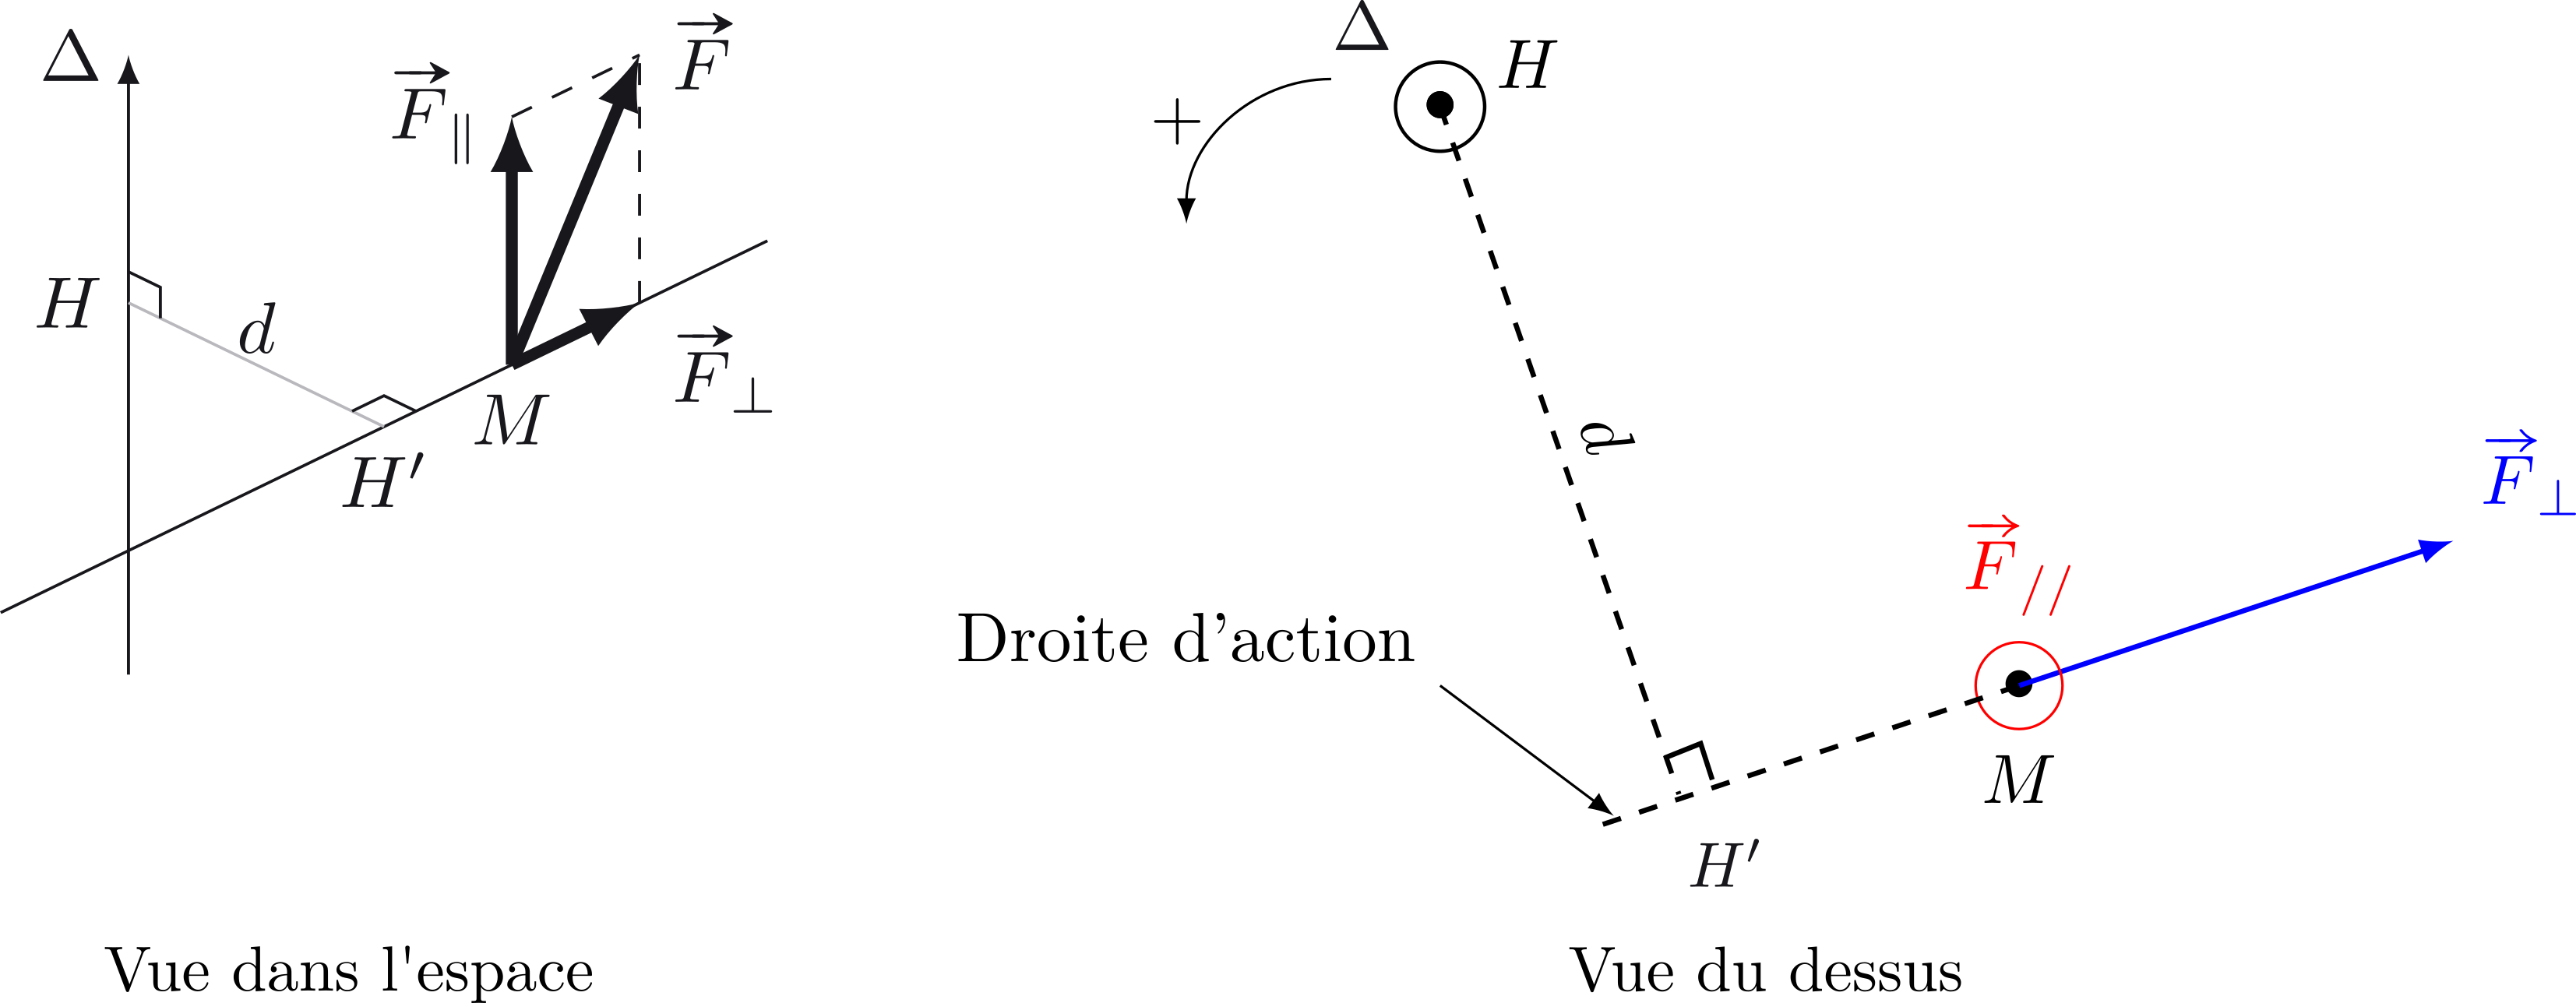
\includegraphics[scale=1, draft=true]{bras_levier}
	}{
		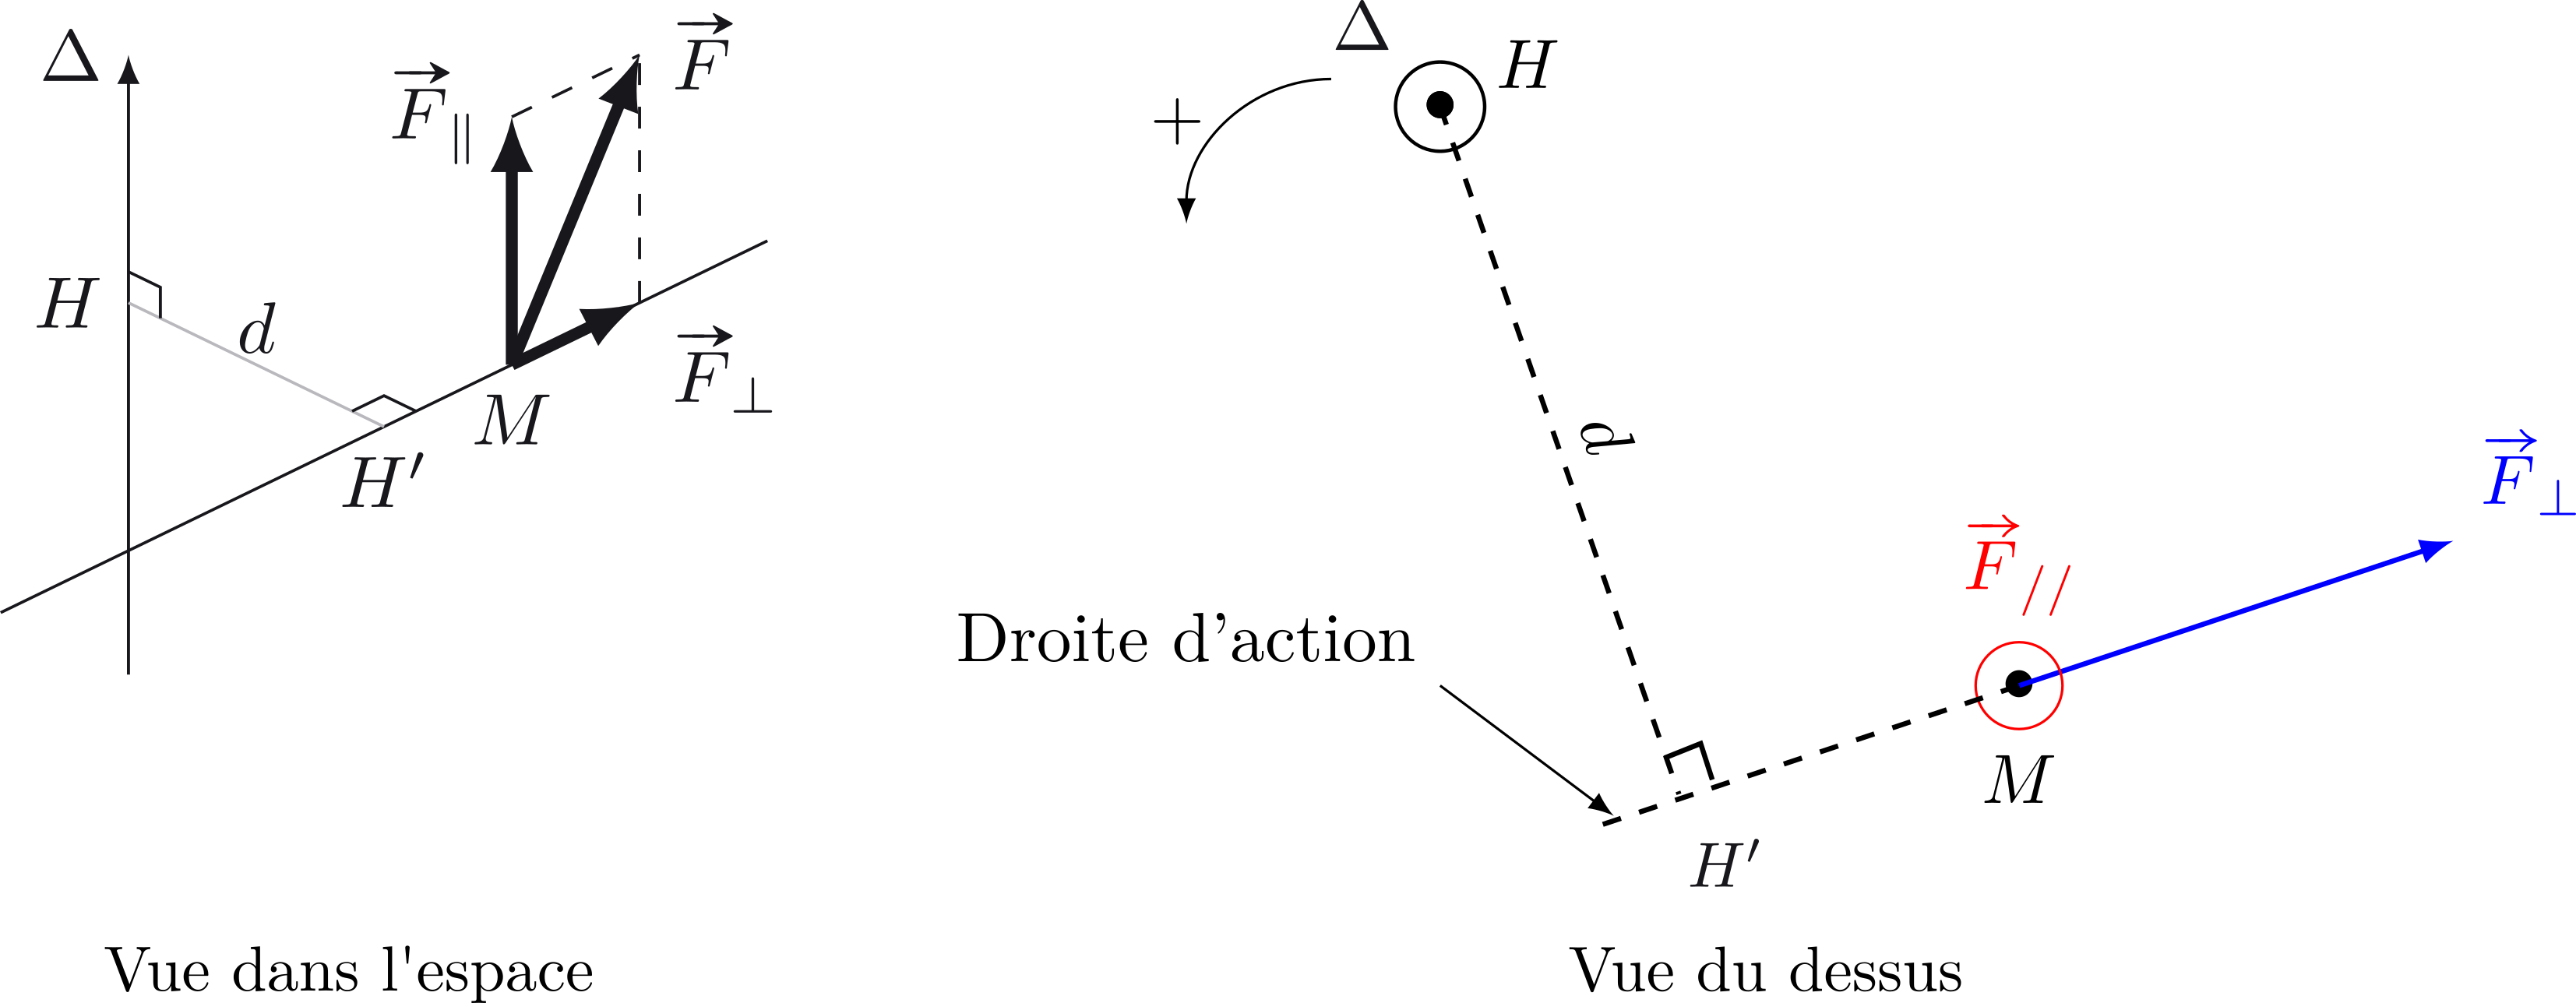
\includegraphics[scale=1]{bras_levier}
	}
	\captionof{figure}{Projection d'une force et bras de levier.}
\end{center}
\begin{tcb*}(prop){Bras de levier d'une force}
	Le \textbf{bras de levier} d'une force $\Ff$ appliquée en un point M est la
	\textbf{distance $d = OH$} entre l'\textbf{axe} de rotation et le
	\textbf{projeté orthogonal H} de O sur la \textbf{droite d'action}, donnée par
	sa composante $\Ff_{\perp}$. Le moment $\Mc_{\D}(\Ff)$ est alors
	\psw{
		\[
			\boxed{
				\Mc_{\D}(\Ff) =
				\OMr \cdot \norm{\Ff_{\perp}} \sin(\a) =
				\pm d\norm{\Ff_{\perp}}
			}
		\]
	}
	On détermine le signe en regardant dans quelle direction la force
	$\Ff_{\perp}$ tend à faire tourner M.
\end{tcb*}
\begin{tcb*}(demo){Bras de levier}
	On commence par déterminer le moment de la force par rapport au point O de
	l'axe, puis on projettera par produit scalaire avec $\ud$. On a donc~:
	\begin{gather*}
		\psw{
			\vv{\rm OM} = \vv{\rm OH} + \vv{\rm HM}
		}
		\qet
		\psw{
			\Ff = \Ff_{\perp} + \Ff_{\parr}
		}
	\end{gather*}
	\begin{DispWithArrows*}
		\Mcf_{\rm O}(\Ff)
		& =
		\psw{
			\vv{\rm OM}\wedge\Ff
		}
		\Arrow{$\Ff = \Ff_{\perp} + \Ff_{\parr}$}
		\\\Lra
		\Mcf_{\rm O}(\Ff)
		& =
		\psw{
			\OM \wedge (\Ff_{\parr} + \Ff_{\perp})
		}
		\Arrow{On distribue}
		\\\Lra
		\Mcf_{\rm O}(\Ff)
		& =
		\psw{
			\underbracket[1pt]{\OM \wedge \Ff_{\parr}}_{\perp \ud} +
			\underbracket[1pt]{\OM \wedge \Ff_{\perp}}_{\parr \ud}
		}
		\CArrow{$\cdot \ud$}
		\\\Ra
		\Mc_{\D}(\Ff)
		& =
		\psw{
			0 +
			\left( \OMr \norm{\Ff_{\perp}}\sin(\a)\ud \right)\cdot \ud
		}
		\Arrow{$\ud \cdot \ud = 1$}
		\\\Lra
		\Aboxed{    \Mc_{\D}(\Ff)
			& =
			\psw{
				\underbracket[1pt]{\OMr \sin(\a)}_{\pm d}\norm{\Ff_{\perp}}
			}}
		\qed
	\end{DispWithArrows*}
\end{tcb*}

\begin{tcb*}[sidebyside](rema)<lftt>{Cas les plus courants}
	\begin{itemize}
		\item En général, $\Ff = \Ff_{\perp}$ donc
		      \psw{
			      \[
				      \OM\wedge\Ff =
				      \underbracket[1pt]{\vv{\rm OH}\wedge\Ff}_{=\pm dF\uz} +
				      \underbracket[1pt]{\vv{\rm HM}\wedge\Ff}_{=\of}
			      \]
		      }
	\end{itemize}
	\vspace{-15pt}
	\begin{center}
		% TODO: Ajouter aire balayée ici ?
		\sswitch{
			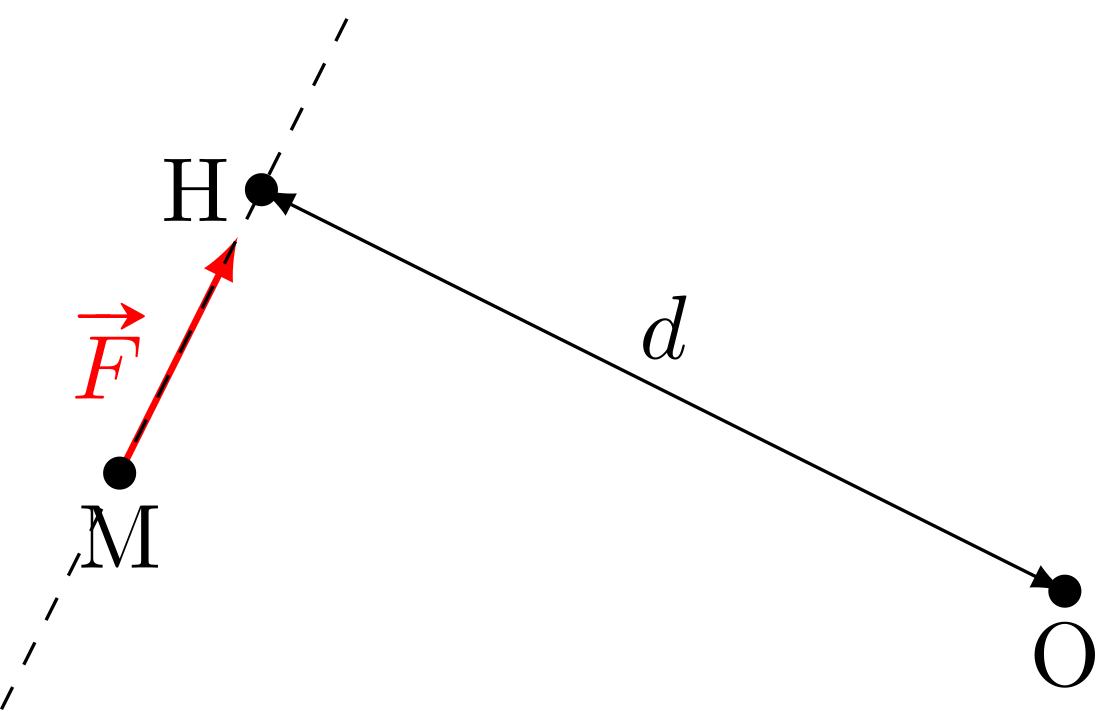
\includegraphics[scale=1, draft=true]{bras_levier-simple}
		}{
			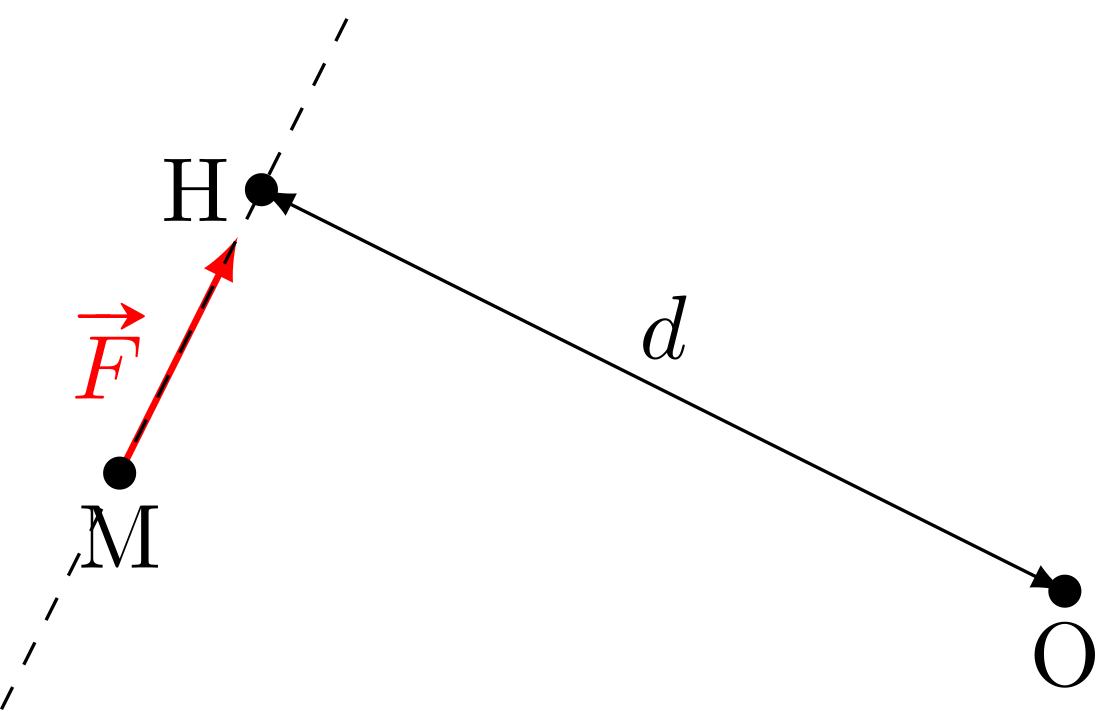
\includegraphics[scale=1]{bras_levier-simple}
		}
		\captionof{figure}{Bras de levier dans le plan $\perp$}
		\label{fig:bras_simple}
	\end{center}
	\tcblower
	\begin{itemize}
		\item \psw{
			      $\Ff \parr \ud \Ra \Mc_{\D} = 0$
		      }
		      et
		      \psw{
			      $\Ff \parr \OM \Ra \Mc_{\D} = 0$
		      }
	\end{itemize}
	\vspace{-15pt}
	\begin{center}
		% TODO: Ajouter aire balayée ici ?
		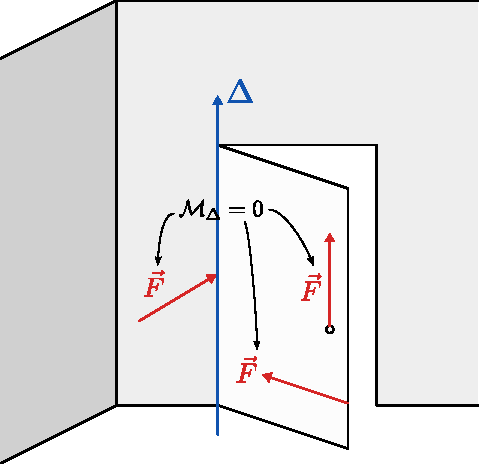
\includegraphics[width=.7\linewidth]{porte_nulles}
		\captionof{figure}{Moments nuls}
		\label{fig:porte_nulles}
	\end{center}
\end{tcb*}

\begin{tcb*}(inte){Moment d'une force et surface balayée}
	On peut interpréter cette valeur comme la surface du parallélépipède
	formé par $\OM$ et $\Ff_{\perp}$ la force dans le plan perpendiculaire à
	l'axe $\D$~: cf.\ Figure~\ref{fig:bras_simple}.
\end{tcb*}

\begin{tcb*}(ror){Méthode du bras de levier}
	\begin{enumerate}
		\item \psw{
			      \textbf{Trouver} le point O de l'axe de rotation dans le plan
			      perpendiculaire à $\ud$ passant par M~;
		      }
		\item \psw{
			      (Optionnel) \textbf{Projeter} $\Ff$ dans ce plan perpendiculaire
			      pour avoir $\Ff_{\perp}$ si nécessaire~;
		      }
		\item \psw{
			      \textbf{Tracer} la droite d'action, passant par M et dirigée par
			      $\Ff_{\perp}$~;
		      }
		\item \psw{
			      \textbf{Placer} le point H et calculer géométriquement $d$~;
		      }
		\item \psw{
			      \textbf{Identifier} le sens de rotation avec la règle de la main
			      droite.
		      }
	\end{enumerate}
\end{tcb*}

\begin{tcb*}[sidebyside](appl)<lftt>{Trois forces pour un mouvement}
	On considère trois forces, de normes égales, exercées sur une porte pour
	l'ouvrir. Laquelle est la plus efficace~? Justifier à l'aide du bras de
	levier.
	\smallbreak
	\hdashrule[0.5ex]{1.1\linewidth}{.5pt}{3pt}
	\begin{enumerate}
		\item \psw{
			      La première force créé un moment
			      \[\Mc_z(\Ff_1) = d_1F\]
		      }
		      \vspace{-15pt}
		\item \psw{
			      La deuxième force créé un moment
			      \[\Mc_z(\Ff_2) = d_2F > d_1F\]
		      }
		      \vspace{-15pt}
		\item \psw{
			      La troisième force créé un moment
			      \[\Mc_z(\Ff_3) = d_2\cos(\theta) < d_2F\]
		      }
		      \vspace{-15pt}
	\end{enumerate}
	\tcblower
	\begin{center}
		\sswitch{
			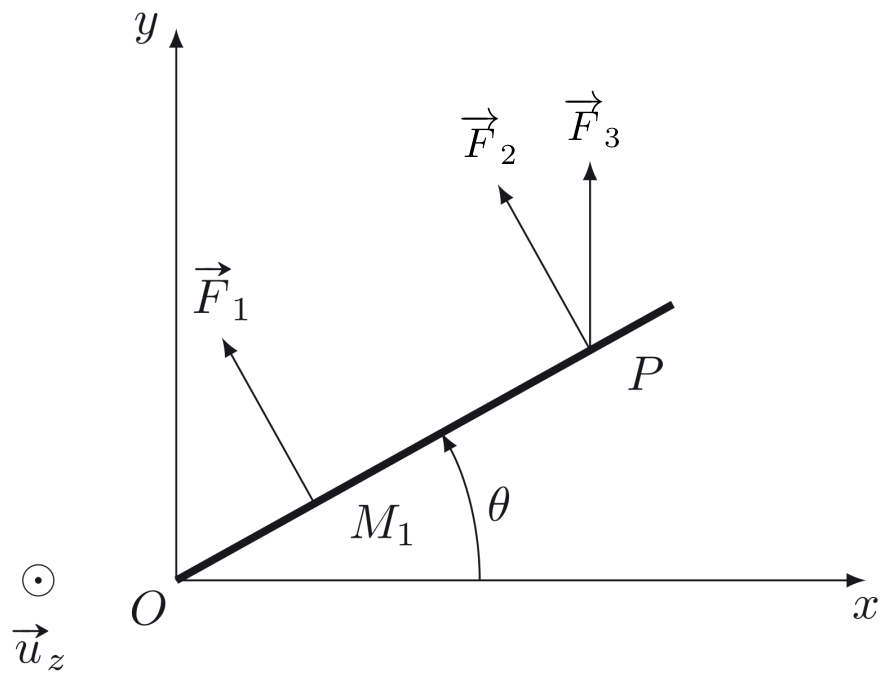
\includegraphics[width=\linewidth]{porte_right}
		}{
			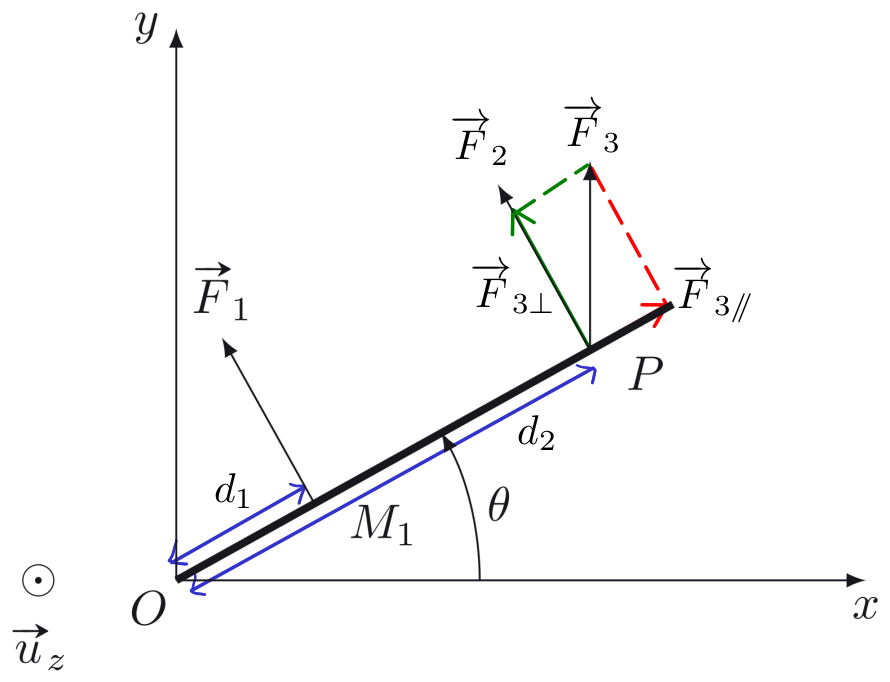
\includegraphics[width=\linewidth]{porte_right-corr}
		}
		\vspace{-15pt}
		\captionof{figure}{Schéma}
		C'est donc \fbox{\psw{$\Ff_2$}} qui est la plus efficace.
	\end{center}
\end{tcb*}

\subsection{Exemples de calcul de moments}

\subsubsection{Clé sur un boulon}
\begin{isd}[lefthand ratio=.45]
	\begin{center}
		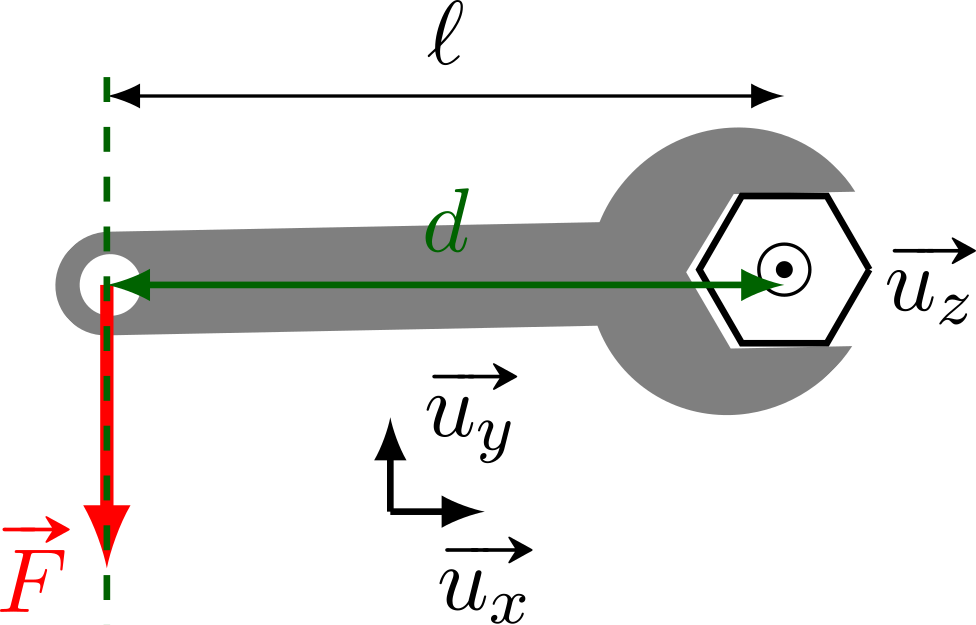
\includegraphics[scale=1]{moment_cle}
	\end{center}
	\tcblower
	\psw{
		\begin{gather*}
			\Ff = -F\uy
			\qqet
			\OM = -\ell\ux
			\\
			\OM\wedge\Ff = \ell F\ux\wedge\uy = \ell F \uz
			\\
			\boxed{\Mc_z(\Ff) = \ell F}
		\end{gather*}
	}
	\vspace{-15pt}
\end{isd}

\subsubsection{Règle à l'horizontale}
\begin{isd}[lefthand ratio=.45]
	\begin{center}
		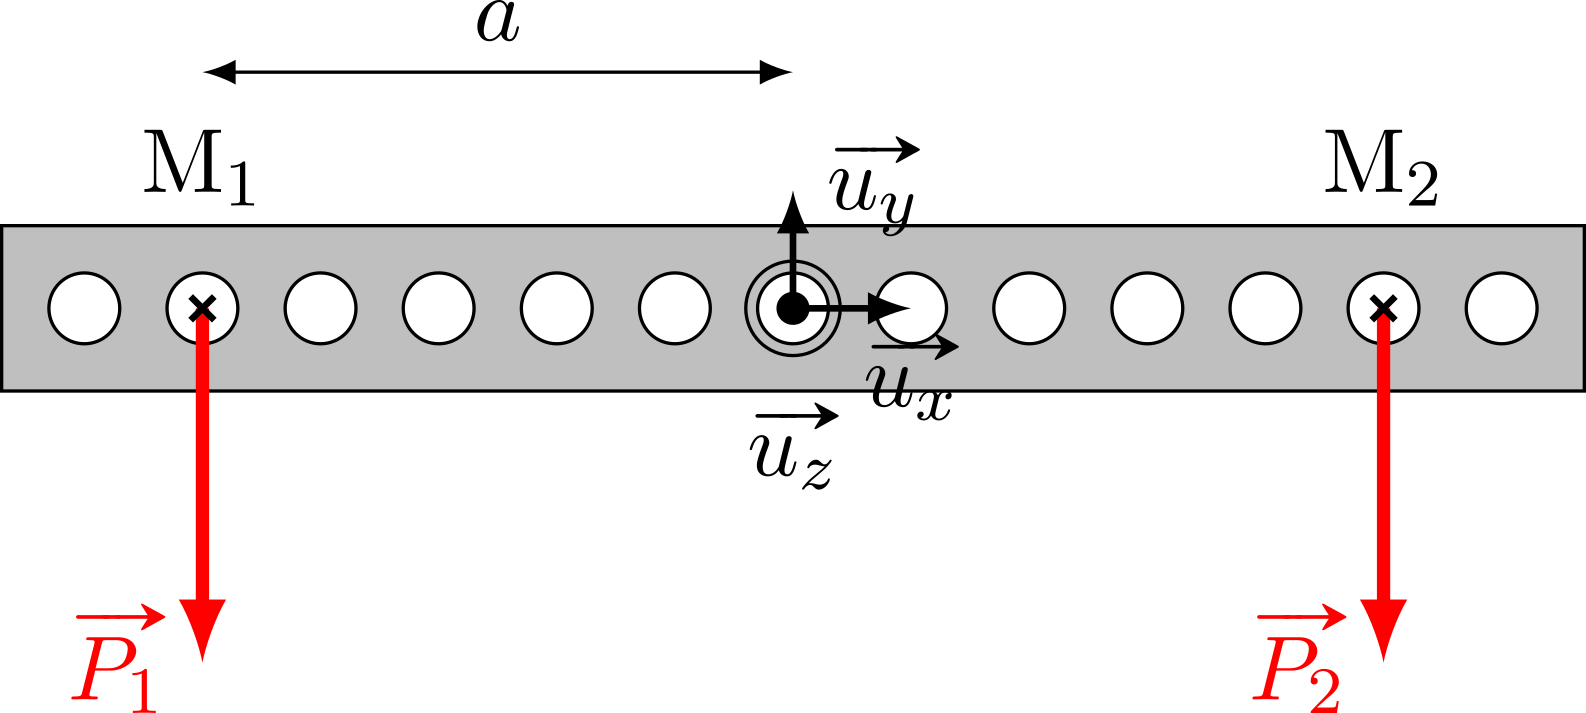
\includegraphics[scale=1]{moment_regle-a}
	\end{center}
	\tcblower
	\psw{
		\begin{gather*}
			\Pf_1 = -mg\uy
			\qqet
			\OM_1 = -a\ux
			\\
			\OM\wedge\Pf_1 = (-a)\times(-mg)\ux\wedge\uy = mga\uz
			\\
			\boxed{\Mc_z(\Pf_1) = mga}
			\qqet
			\boxed{\Mc_z(\Pf_2) = -mga}
		\end{gather*}
		\centering La règle ne tourne pas.
	}
\end{isd}

\section{Moment cinétique}
Comme pour le chapitre de mécanique énergétique, on a commencé par introduire le
concept de travail d'une force avant de l'appliquer sous une certaine forme à
l'énergie cinétique du corps. Ici, on a défini le moment d'une force,
caractérisant sa capacité à faire tourner un point~: il paraît donc naturel de
définir une grandeur vectorielle caractérisant la rotation d'un point matériel~:
c'est le \textbf{moment cinétique}.

\subsection{Moment cinétique par rapport à un point}
\begin{tcb*}[sidebyside, righthand ratio=.2](defi){Moment \textbf{cinétique} par
			rapport à un point}
	Le moment cinétique d'un point M par rapport à un point O dans le
	référentiel $\Rc$ est le \textbf{vecteur}~:
	\psw{
		\[
			\boxed{\Lcf_{\Or/\Rc}(\Mr) = \OM\wedge\pf_{\Mr/\Rc} = \OM\wedge
				m\vf_{\Mr/\Rc}}
		\]
	}%
	qui traduit la «~quantité de rotation~» d'un point matériel en rotation
	autour d'un autre.
	\tcblower
	\tcbsubtitle{\fatbox{\textbf{Unité}}}
	\[
		\psw{
			\si{N.m.s} = \si{J.s}
		}
	\]
\end{tcb*}

\begin{tcb*}[breakable](inte){Moment cinétique~: information et géométrie}
	\begin{itemize}
		\item Considérons un repère polaire autour de l'axe
		      $(\Or z)$. On a alors
		      \psw{
			      \[
				      \left\{
				      \begin{aligned}
					      \OM & = r\ur            \\
					      \vf & = \rp\ur + r\w\ut
				      \end{aligned}
				      \right.
				      \quad\Ra\quad
				      \Lcf_{\Or/\Rc} = (r\ur)\wedge m(\rp\ur+r\w\ut) = mr^2\w\uz
			      \]
		      }%
		      Ainsi, \textbf{le moment cinétique ne conserve une information que sur
			      la rotation du système}. Si celui-ci est nul tout le temps, soit il
		      n'y a pas de mouvement, soit le vecteur vitesse et le vecteur position
		      sont colinéaires et le mouvement est rectiligne.
		\item La \textbf{direction} de $\Lcf_{\Or}$
		      indique la manière dont M tourne autour de O.
	\end{itemize}
	\begin{center}
		\begin{tabularx}{\linewidth}{Y|Y|Y}
			\sswitch{
				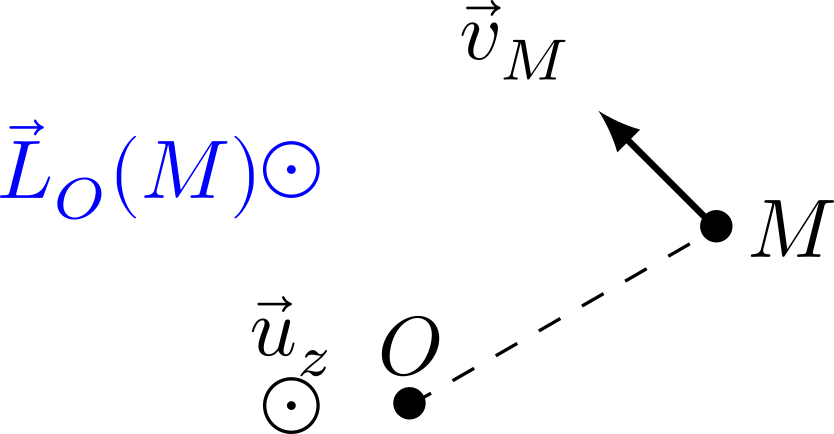
\includegraphics[scale=1, draft=true]{moment_cin-a}
			}{
				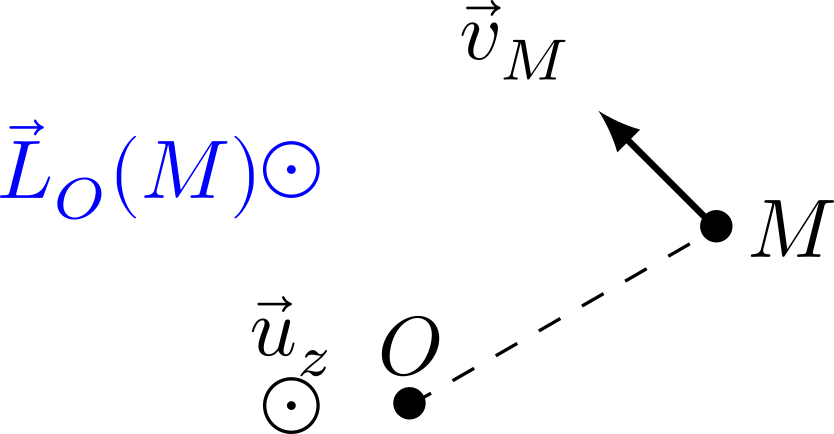
\includegraphics[scale=1]{moment_cin-a}
			}
			 &
			\sswitch{
				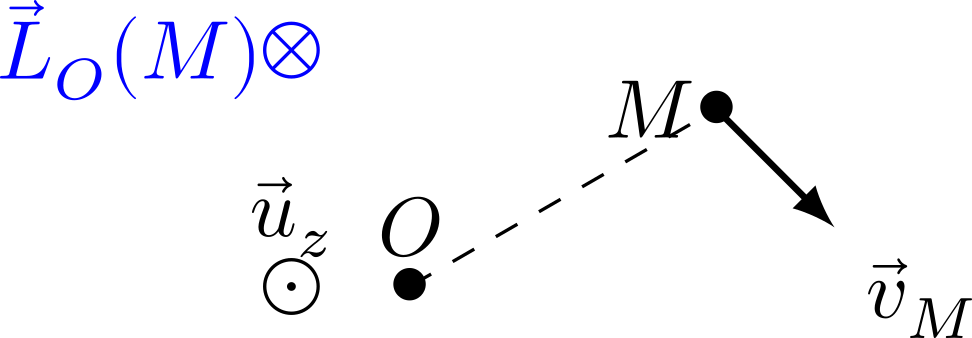
\includegraphics[scale=1, draft=true]{moment_cin-b}
			}{
				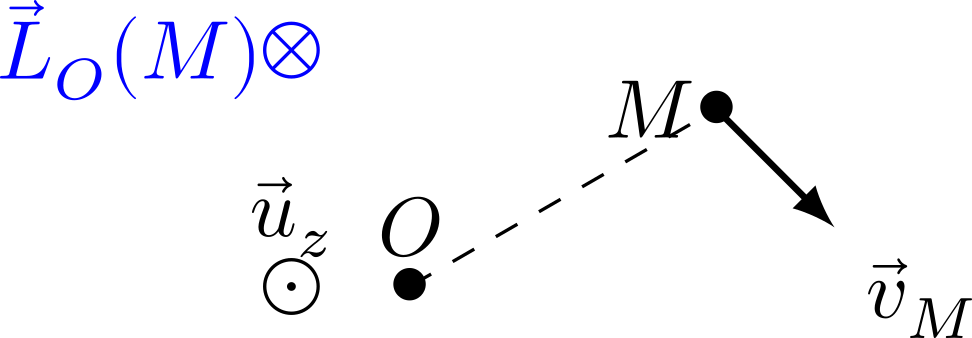
\includegraphics[scale=1]{moment_cin-b}
			}
			 &
			\sswitch{
				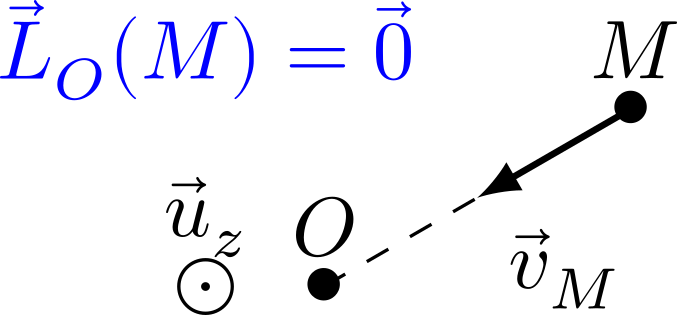
\includegraphics[scale=1, draft=true]{moment_cin-c}
			}{
				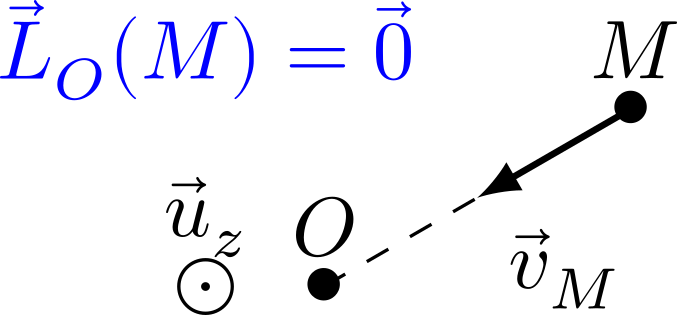
\includegraphics[scale=1]{moment_cin-c}
			}
			\\
			\psw{
				Si $\Lcf_{\Or}(\Mr)$ est dirigé selon $+\uz$, M tourne autour de O dans
				le sens \textbf{direct}.
			}
			 &
			\psw{
				Si $\Lcf_{\Or}(\Mr)$ est dirigé selon $-\uz$, M tourne autour de O dans
				le sens \textbf{horaire}.
			}
			 &
			\psw{
				Si $\Lcf_{\Or}(\Mr) = \of$, M ne tourne pas autour du point O.
			}
		\end{tabularx}
	\end{center}
\end{tcb*}

\begin{tcb*}(rema)<lftt>'l'{Conséquences du moment cinétique}
	\begin{enumerate}
		\item Le vecteur $\Lcf_{\Or}$ est orthogonal à $\OM$ et à $\vf$.
		\item Le moment cinétique $\Lcf_{\Or}$ dépend du point O~:
		      \[
			      \boxed{\Lcf_{\Or'}(\Mr) = \Lcf_{\Or}(\Mr) + \vv{\rm O'O}\wedge
				      m\vf}
		      \]
	\end{enumerate}
\end{tcb*}

\subsection{Moment cinétique par rapport à un axe \xul{orienté}}
\begin{tcb*}[sidebyside, righthand ratio=.2](defi){Moment cinétique par rapport
			à un axe orienté}
	Le moment cinétique d'un point M par rapport à un axe orienté $\D$
	dans le référentiel $\Rc$ est le \textbf{scalaire}~:
	\psw{
		\[
			\boxed{\Lc_{\D}(\Mr) = (\OM\wedge\pf_{\Mr/\Rc})\cdot\ud =
				\Lcf_{\Or/\Rc}(\Mr)\cdot\ud}
		\]
	}%
	avec O un point de l'axe. $\Lc_{\D}$ est le projeté du moment
	$\Lcf_{\Or/\Rc}$ sur $\D$.
	\tcblower
	\tcbsubtitle{\fatbox{\textbf{Unité}}}
	\psw{
		\[
			\si{J.s}
		\]
	}
\end{tcb*}

Cette fois-ci aussi, c'est le \textbf{signe} de $\Lc_{\D}$ qui indique le sens de
rotation de M autour de l'axe~: s'il est \textbf{positif} il se fait dans le
sens \textbf{direct}.

\begin{tcb*}[cnt, bld](impo)<lftt>'l'{Moment vecteur et moment scalaire}
	$\Lc_{\D}$ est un scalaire, alors que $\Lcf_{\Or}$ est un vecteur~!
\end{tcb*}

\begin{tcb*}[cnt](prop){Moment cinétique scalaire et point d'origine}
	$\Lc_{\D}$ est indépendant du point O de l'axe $\D$.
\end{tcb*}
\begin{tcb*}(demo){Moment cinétique scalaire et point d'origine}
	\psw{
		\[
			\Lcf_{\mathrm{O'}/\Rc}\cdot\ud =
			\left[(\vv{\rm O'O}+\OM)\wedge\pf_{\Mr/\Rc}\right]\cdot\ud =
			\underbracket[1pt]{
				(\underbracket[1pt]{\vv{\rm O'O}}_{\parr\ud}\wedge\pf_{\Mr/\Rc})
				\cdot\ud}_{=0}
			+ \Lcf_{\Or/\Rc}\cdot\ud = \Lcf_{\Or/\Rc}\cdot\ud
		\]
	}
	\vspace{-15pt}
\end{tcb*}

\section{Théorème du moment cinétique}
Rien que par les unités des différentes grandeurs, on peut imaginer le lien
entre moment cinétique et moment d'une force, ou avec un peu de recule sur ce
qu'il est en train de se passer…

\subsection{Par rapport à un point \textit{fixe}}
\begin{tcb*}(theo){Théorème du moment cinétique par rapport à un point
			\textit{fixe}}
	Pour un point matériel M de masse $m$ soumis à des forces extérieures
	$\Ff_i$ dans un référentiel $\Rc$ supposé galiléen et O un point
	\textbf{fixe} dans $\Rc$, on a
	\psw{
		\[\boxed{\dv{\Lcf_{\Or/\Rc}(\Mr)}{t} = \sum_i\Mcf_{\Or}(\Ff_i)}\]
	}
\end{tcb*}
\begin{tcb*}(demo){TMC vectoriel}
	Comme pour le TPC où l'on applique $\cdot\vf$ sur le PFD, il suffit ici
	d'appliquer $\OM\wedge$~:
	\smallbreak
	\begin{isd}
		On part du PFD
		\begin{DispWithArrows*}[fleqn, mathindent=10pt]
			\psw{m\af} & = \psw{\sum_i \Ff_i}
			\Arrow{$\pf = m\vf$}
			\\\Lra
			\psw{\dv{\pf}{t}}          & = \psw{\sum_i\Ff_i}
			\CArrow{$\OM \wedge \cdot $}
			\\\Ra
			\psw{\OM\wedge\dv{\pf}{t}} & =
			\psw{\OM\tikzmark{om}\wedge\sum_i\tikzmark{ff}\Ff_i}
		\end{DispWithArrows*}
		\tcblower
		\begin{align*}
			\psw{\dv{\Lcf_{\Or/\Rc}(\Mr)}{t}}
			 & =
			\psw{
				\dv{\tikzmark{dv}}{t}
				\left(\OM\tikzmark{omd}
				\wedge\pf\tikzmark{pfd}
				\right)
			}
			\\\Lra
			\psw{\dv{\Lcf_{\Or/\Rc}(\Mr)}{t}}
			 & =
			\psw{
				\underbracket[1pt]{
					\xunderbracket{\dv{\OM}{t}}_{\parr\vf}
					\wedge
					\xunderbracket{\pf}_{\parr\vf}
				}_{=\of}
				+ \OM\wedge\dv{\pf}{t}
			}
		\end{align*}
	\end{isd}
	\begin{gather*}
		\beforetext{Ainsi,}
		\psw{
			\dv{\Lcf_{\Or/\Rc}(\Mr)}{t} = \sum_i\OM\wedge\Ff_i
			\Lra
			\boxed{\dv{\Lcf_{\Or/\Rc}(\Mr)}{t} = \sum_i\Mcf_{\Or}(\Ff_i)}
		}
		\qed
	\end{gather*}
\end{tcb*}
\tikz[remember picture, overlay]
\draw[-stealth, transform canvas={yshift=12pt}, color=\sswitch{white}{black}]
([shift={(-6pt,0)}]pic cs:om) to[out=90, in=90] (pic cs:ff)
;
\tikz[remember picture, overlay]
\draw[-stealth, transform canvas={yshift=6pt}, color=\sswitch{white}{black}]
(pic cs:dv) to[out=90, in=90] ([shift={(-6pt,6pt)}]pic cs:omd)
;
\tikz[remember picture, overlay]
\draw[-stealth, transform canvas={yshift=6pt}, color=\sswitch{white}{black}]
(pic cs:dv) to[out=90, in=90] ([shift={(-6pt,6pt)}]pic cs:pfd)
;
\vspace{-20pt}

\subsection{Par rapport à un axe \xul{orienté} \textit{fixe}}
\begin{tcb*}(theo){Théorème du moment cinétique par rapport à un axe
			\xul{orienté} \textit{fixe}}
	Pour un point matériel M de masse $m$ soumis à des forces extérieures
	$\Ff_i$ dans un référentiel $\Rc$ supposé galiléen et $\D$ un axe
	orienté \textbf{fixe} dans $\Rc$, on a
	\psw{
		\[\boxed{\dv{\Lc_{\D}(\Mr)}{t} = \sum_i\Mc_{\D}(\Ff_i)}\]
	}
	\vspace{-15pt}
\end{tcb*}
\begin{tcb*}(demo){TMC scalaire}
	On projette simplement le TMC version vectorielle sur $\ud$~:
	\psw{
		\begin{align*}
			\dv{\Lcf_{\Or/\Rc}(\Mr)}{t}\cdot\ud & = \sum_i\Mcf_{\Or}(\Ff_i)\cdot\ud
			\\\Lra
			\dv{\Lcf_{\Or/\Rc}(\Mr)\cdot\ud}{t} & = \sum_i\Mc_d(\Ff_i)
			\\\Lra
			\Aboxed{\dv{\Lc_d(\Mr)}{t}          & = \sum_i\Mc_d(\Ff_i)}
			\qed
		\end{align*}
	}
\end{tcb*}

\section{Exemple du pendule simple}
\hspace*{-0.75cm}
\begin{minipage}{0.70\linewidth}
	\begin{enumerate}[label=\sqenumi]
		\bitem{De quoi parle-t-on~?} On étudie le mouvement d'une masse
		suspendue à un fil, dans $\Rc\ind{laboratoire}$ supposé galiléen.
		\bitem{Schéma}.
		\bitem{Modélisation.} On choisit d'utiliser des coordonnées polaires.
		\begin{itemize}
			\item La masse est assimilée à un point matériel M.
			\item Origine~: point d'accroche du fil (centre de rotation
			      pendule).
			\item Repère~: $(O,\ur,\ut)$ avec base polaire (voir schéma).
			\item Repérage~: $\OM = \ell\ur$, $\vf = \ell\tp\ut$.
			\item $t$ initial~: moment du lâché, $\th(0) = \th_0$ et
			      $\th(0) = 0$.
		\end{itemize}
	\end{enumerate}
\end{minipage}
\hfill
\begin{minipage}{0.25\linewidth}
	\begin{center}
		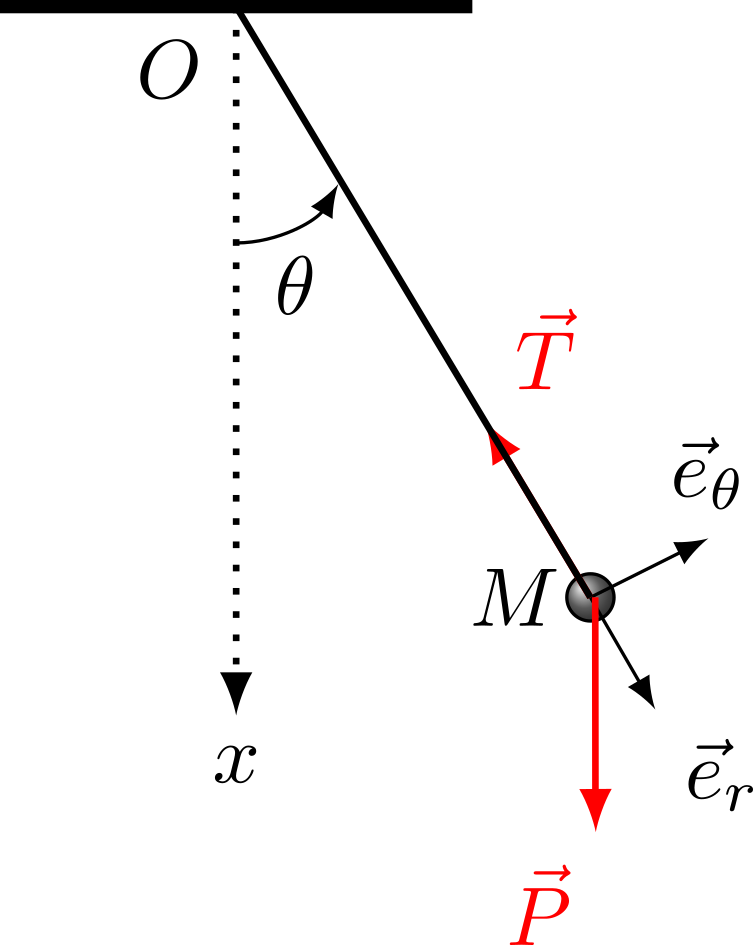
\includegraphics[width=\linewidth]{pendule_plain}
		\captionof{figure}{Pendule simple.}
	\end{center}
\end{minipage}
\begin{enumerate}[label=\sqenumi, start=4]
	\bitem{Bilan des forces.}
	\psw{
		\[
			\begin{array}{ll}
				\textbf{Poids}   & \Pf = m\gf = mg(\cos\th \ur - \sin\th \ut) \\
				\textbf{Tension} & \Tf = -T\ur
			\end{array}
		\]
	}
	\bitem{Calcul des moments.}
	\psw{
		\[
			\left\{
			\begin{array}{rcl}
				\Mcf_{\Or}(\Pf) & = & (\ell\ur)\wedge mg(\cos\th \ur - \sin\th \ut)
				= -mg\ell\sin\th\uz                                                 \\
				\Mcf_{\Or}(\Tf) & = & (\ell\ur)\wedge(-T\ur) = \of                  \\
				\Lcf_{\Or}(\Mr) & = & (\ell\ur)\wedge(m\ell\tp\ut) =
				m\ell^2\tp\uz
			\end{array}
			\right.
		\]
	}
	Ainsi
	\psw{
		\[
			\boxed{\Mc_z(\Pf) = -mg\ell\sin\th}
			\qqet
			\boxed{\Mc_z(\Tf) = 0}
			\qqet
			\boxed{\Lc_z(\Mr) = m\ell^2\tp}
		\]
	}
	\vspace{-15pt}
	\bitem{TMC}~:
	\psw{
		\begin{align*}
			m\ell^2\tpp                          & = -mg\ell\sin\th + 0
			\\\Lra
			\Aboxed{\tpp + \frac{g}{\ell}\sin\th & = 0}
			\qed
		\end{align*}
	}
\end{enumerate}
On a donc bien retrouvé l'équation du mouvement du pendule simple~!

\end{document}
